%%%%%%%%%%%%%%%%%%%%%%%%%% EDP Science %%%%%%%%%%%%%%%%%%%%%%%%%%%%
%
%%%\documentclass[option]{webofc}
%%% "twocolumn" for typesetting an article in two columns format (default one column)
%

\documentclass[onecolumn]{webofc}
\usepackage[varg]{txfonts}   % Web of Conferences font
\usepackage[none]{hyphenat} % Remove hyphens
\usepackage{indentfirst}
\usepackage{setspace}
\usepackage{listings}
\usepackage[superscript]{cite}
\graphicspath{{graphics/}{graphics/arch/}{Graphics/}{./}} % Look in these folders for graphics
%
%
% Put here some packages required or/and some personal commands
\renewcommand{\thesection}{\Roman{section}.}
\renewcommand{\thesubsection}{\Alph{subsection}.}
\renewcommand{\bibsection}{\section{REFERENCES}}
\addto\captionsenglish{\renewcommand{\figurename}{FIG.}}

\lstset{frame=tb,
  aboveskip=3mm,
  belowskip=3mm,
  showstringspaces=false,
  columns=flexible,
  basicstyle={\small\ttfamily},
  numbers=none,
  numberstyle=\tiny\color{gray},
  keywordstyle=\color{blue},
  commentstyle=\color{dkgreen},
  stringstyle=\color{mauve},
  breaklines=true,
  breakatwhitespace=true,
  tabsize=3
}

%
%
\begin{document}
%
% TODO
\title{Gram-Schmidt and the QR algorithm}
%
% subtitle is optional
%
%%%\subtitle{Do you have a subtitle?\\ If so, write it here}

\author{\firstname{Arleth} \lastname{Salinas}\\\small{University of Chicago, Chicago, Illinois 60637}
%\fnsep\thanks{\email{Mail address for firstauthor}} \and
        %\firstname{Second author} \lastname{Second author}\inst{2}\fnsep\thanks{\email{Mail address for second
        %     author if necessary}} \and
        %\firstname{Third author} \lastname{Third author}\inst{3}\fnsep\thanks{\email{Mail address for last
             %author if necessary}}
        % etc.
}
%\and
%           the second here 
%\and
%           Last address

\abstract{%

}
%
\maketitle
% \thispagestyle{plain}
% \fancyfoot[C]{\thispage}
%
\section{INTRODUCTION}
\label{intro}
In this expository, we will explore the QR algorithm and the linear algebra ideas behind it. The QR algorithm was developed by John Francis and published in \textit{The Computer Journal} in 1961\cite{RefA}.  This algorithm is powerful as it can be used to calculate the eigenvalue and eigenvectors of a matrix. We will begin by establishing the linear algebra ideas, namely the Gram-Schmidt process and QR decomposition, needed to execute the QR algorithm. We will give examples of these linear algebra ideas, then discuss an actual implementation of the QR algorithm as well as some results from experiments with the algorithm.


\section{MATHEMATICAL DERIVATIONS}
\subsection{Gram-Schmidt Algorithm}
\subsubsection*{Background}
The Gram-Schmidt algorithm is named after Erhard Schmidt and J.P. Gram. Gram published his paper on the algorithm in 1883, and Schmidt based his version of the procedure on Schmidt's original paper. This algorithm was also independently found by P.S. Laplace, appearing in a paper he published in 1820. We will proceed to describe the Gram-Schmidt process\cite{RefB}.

\subsubsection*{The Algorithm}
Let $\mathbf{X} = \mathbf{x}_1, \mathbf{x}_2, \ldots, \mathbf{x}_n$ be a linearly independent system.

Gram-Schmidt constructs an orthonormal basis $\mathbf{v}_1, \mathbf{v}_2, \ldots, \mathbf{v}_n$ such that $$\text{span}\{\mathbf{x}_1, \mathbf{x}_2, \ldots, \mathbf{x}_n\}= \text{span}\{\mathbf{v}_1, \mathbf{v}_2, \ldots, \mathbf{v}_n\}.$$

For the first step of the process, initialize $$\mathbf{v}_1= \mathbf{x}_1, \mathbf{e}_1 = \frac{\mathbf{v}_1}{\|\mathbf{v}_1\|}.$$

The next step, set $$\mathbf{v}_2 = \mathbf{x}_2 - \text{proj}_{\mathbf{v}_1}(\mathbf{x}_2), \mathbf{e}_2 = \frac{\mathbf{v}_2}{\|\mathbf{v}_2\|}.$$

Note, we define $\text{proj}_{\mathbf{x}}(\mathbf{v})$ as $$\text{proj}_{\mathbf{x}}(\mathbf{v}) = \frac{\mathbf{x} \cdot \mathbf{v}}{\|\mathbf{v}\|^{2}}\mathbf{v}$$

The 3rd step, set $$\mathbf{v}_3 = \mathbf{x}_3 - \text{proj}_{\mathbf{v}_1}(\mathbf{x}_3) - \text{proj}_{\mathbf{v}_2}(\mathbf{x}_3), \mathbf{e}_2 = \frac{\mathbf{v}_3}{\|\mathbf{v}_3\|}.$$

We can continue this process $n$ times,  setting,

$$\mathbf{v}_n = \mathbf{x}_n - \text{proj}_{\mathbf{v}_1}(\mathbf{x}_n) - \text{proj}_{\mathbf{v}_2}(\mathbf{x}_n)- \ldots - \text{proj}_{\mathbf{v}_n-1}(\mathbf{x}_n), \mathbf{e}_n = \frac{\mathbf{v}_n}{\|\mathbf{v}_n\|}$$.

We end with vectors $\mathbf{e}_1, \mathbf{e}_2, \ldots, \mathbf{e}_n$ which are the vectors of our orthonormal basis for $\mathbf{X}$. 

We can reformulate the above and see that to find $\mathbf{v}_k$, we can do the following,
$$\mathbf{v}_k = \mathbf{x}_k - \sum_{j=1}^{n-1}\text{proj}_{\mathbf{v}_j}(\mathbf{x}_k).$$

\subsubsection*{Example}
Let $$\mathbf{X} =  \begin{bmatrix}
1 & 1 \\
2 & -1 \\
-2 & 4 
\end{bmatrix}. $$

We would set, $$\mathbf{v}_1 = \begin{bmatrix} 1 & 2 & -2 \end{bmatrix}^{\top}$$
$$\mathbf{v}_1  = \frac{\mathbf{v}_1 }{\sqrt[]{1+1+4}} = \frac{\mathbf{v}_1 }{3} = \begin{bmatrix}
\frac{1}{3} && \frac{2}{3} && -\frac{2}{3}
\end{bmatrix}^{\top}$$

Then, to find the second orthonormal vector in the basis, we do,
$$\mathbf{v}_2 = \mathbf{x}_2 - \text{proj}_{\mathbf{v}_1}\mathbf{x}_2 = \mathbf{x}_2 - \text{proj}_{\mathbf{v}_1}\mathbf{x}_2 = \frac{\mathbf{x}_2 \cdot \mathbf{v}_1}{\|\mathbf{v}_1\|^{2}}\mathbf{v}_1 = \begin{bmatrix}
2 && 1 && 2
\end{bmatrix}^{\top}$$

Normalizing $\mathbf{v}_2$ we get $$\begin{bmatrix}
\frac{2}{3} && \frac{1}{3} && \frac{2}{3}
\end{bmatrix}^{\top}$$

So, our orthonormal basis for the matrix $\mathbf{X}$ is $$\left\{
\begin{pmatrix} \frac{1}{3} \\ \frac{2}{3} \\ -\frac{2}{3} \end{pmatrix},
\begin{pmatrix} \frac{2}{3} \\ \frac{1}{3} \\ \frac{2}{3}\end{pmatrix}
\right\}$$

\subsection{QR Decomposition}
\subsubsection*{Background}
To use the QR algorithm, we must first introduce the QR decomposition. This decomposition was developed by John Francis while making modifications to Rutishauser's algorithm for finding eigenvalues, which involved using the LR decomposition. The QR decomposition relies on knowing that a matrix can be reduced to a triangular matrix, thanks to Schur\cite{RefA}.

\subsubsection*{QR Decomposition Statement}
For any matrix $\mathbf{A}$ (of order n, say) there exists a unitary matrix $\mathbf{Q}$ such that $\mathbf{A} = \mathbf{QR}$ where $\mathbf{R}$ is an upper (right) triangular matrix which has real, non-negative, diagonal elements. Moreover, $\mathbf{Q}$ is unique if $\mathbf{A}$ is non-singular.

\subsubsection*{Obtaining the QR Decomposition}
\textbf{Via Gram-Schmidt}

One method of obtaining the QR decomposition is by using the Gram-Schmidt algorithm. 

Let $\mathbf{X} = \mathbf{x}_1, \mathbf{x}_2, \ldots, \mathbf{x}_n$ be a linearly independent system.

For the first step of the process, initialize $$\mathbf{v}_1= \mathbf{x}_1, \mathbf{e}_1 = \frac{\mathbf{v}_1}{\|\mathbf{v}_1\|}.$$

The next step, set $$\mathbf{v}_2 = \mathbf{x}_2 - \text{proj}_{\mathbf{v}_1}(\mathbf{x}_2), \mathbf{e}_2 = \frac{\mathbf{v}_2}{\|\mathbf{v}_2\|}.$$

The 3rd step, set $$\mathbf{v}_3 = \mathbf{x}_3 - \text{proj}_{\mathbf{v}_1}(\mathbf{x}_3) - \text{proj}_{\mathbf{v}_2}(\mathbf{x}_3), \mathbf{e}_2 = \frac{\mathbf{v}_3}{\|\mathbf{v}_3\|}.$$

We can continue this process $n$ times,  setting,

$$\mathbf{v}_n = \mathbf{x}_n - \text{proj}_{\mathbf{v}_1}(\mathbf{x}_n) - \text{proj}_{\mathbf{v}_2}(\mathbf{x}_n)- \ldots - \text{proj}_{\mathbf{v}_n-1}(\mathbf{x}_n), \mathbf{e}_n = \frac{\mathbf{v}_n}{\|\mathbf{v}_n\|}$$.

To obtain the QR decomposition, we define the matrices $\mathbf{Q}, \mathbf{R}$ as,
$$\mathbf{Q} = [\mathbf{e}_1 | \mathbf{e}_2 | \ldots | \mathbf{e}_n], \mathbf{R} = \begin{bmatrix}
  \mathbf{e}_1 \cdot \mathbf{x}_1 &
  \mathbf{e}_1 \cdot \mathbf{x}_2 &
  \mathbf{e}_1 \cdot \mathbf{x}_3 & \cdots \\
                                         0 &
 \mathbf{e}_2 \cdot \mathbf{x}_2 &
 \mathbf{e}_2 \cdot \mathbf{x}_3& \cdots \\
                                         0 &
                                         0 &
  \mathbf{e}_3 \cdot \mathbf{x}_3& \cdots \\
                                    \vdots &
                                    \vdots &
                                    \vdots &
                                    \ddots\end{bmatrix}.$$
\\
\textbf{Other methods}
\\
Other methods that can be used to obtain the QR decomposition include using Householder reflections which involve taking a vector and rotating it about a plane or hyperplane\cite{RefC}. A benefit of using Householder reflections over the Gram-Schmidt process is, Gram-Schmidt experiences numerical instability. This is because round-off error can occur as vectors are projected onto each orthonormal basis vector 

One can also use Givens rotations. This involves rotating the matrix and zero-ing each element below the diagonal of the matrix, which forms the $\mathbf{R}$ matrix. Concatenating all of the Givens rotations forms the $\mathbf{Q}$ matrix\cite{RefD}.


\subsection{QR Algorithm}
\subsubsection*{The Algorithm}
Now that we have established the QR decomposition, we can proceed to how the QR decomposition can be used in the QR algorithm. 

Let $\mathbf{X} = \mathbf{x}_1, \mathbf{x}_2, \ldots, \mathbf{x}_n$ be a linearly independent system.

Initialize $\mathbf{X}_1 = \mathbf{X}$ .
$$\mathbf{X}_1 = \mathbf{Q}_1\mathbf{R}_1$$
$$\mathbf{R}_1\mathbf{Q}_1 = \mathbf{X}_2 = \mathbf{Q}_2\mathbf{R}_2$$
$$\mathbf{R}_2\mathbf{Q}_2 = \mathbf{X}_3 = \mathbf{Q}_3\mathbf{R}_3$$
$$\vdots$$
$$\mathbf{R}_{k-1}\mathbf{Q}_{k-1} = \mathbf{X}_k = \mathbf{Q}_k\mathbf{R}_k$$

As we repeat this process, if $\mathbf{A}$ is non-singular (has a determinant of 0) then the elements below the diagonal of $\mathbf{X}_k$ tend to $0$, the elements above the diagonal tend to fixed values, and the elements on the principal diagonal then to the eigenvalues of $\mathbf{A}$.

\subsubsection*{Example}
Recall the matrix,
$$\mathbf{X} =  \begin{bmatrix}
1 & 1 \\
2 & -1 \\
-2 & 4 
\end{bmatrix}. $$

and the process we undertook to find an orthonormal basis for the matrix using the Gram-Schmidt process.

In particular, we can construct the $\mathbf{QR}$ decomposition using the basis vectors we obtained:
$$\left\{
\begin{pmatrix} \frac{1}{3} \\ \frac{2}{3} \\ -\frac{2}{3} \end{pmatrix},
\begin{pmatrix} \frac{2}{3} \\ \frac{1}{3} \\ \frac{2}{3}\end{pmatrix}
\right\}$$

We simply define Q to have its columns be the corresponding basis vectors as follows:
$$\mathbf{Q} = 
\begin{bmatrix}
\frac{1}{3} & \frac{2}{3} \\
\frac{2}{3} & \frac{1}{3} \\
-\frac{2}{3} & \frac{2}{3} 
\end{bmatrix}.$$

And R will be:
$$\mathbf{R} = 
\begin{bmatrix}
3 & -3 \\
0 & 3 \\
\end{bmatrix}.$$
where we simply took the dot products of the basis vectors with the vectors of the matrix $\mathbf{X}$.

\section{IMPLEMENTATION}

\subsection{Background}
The implementation was done in the Julia programming language. We will proceed to show the code and discuss important implementation decisions made in the implementation of the QR algorithm and its precursory components.

\subsection{Gram-Schmidt and QR Decomposition}
\begin{lstlisting}
"""
Compute an orthonormal basis for a full-rank, real, 
square matrix of any size
Inputs:
    x - matrix to find orthonormal basis and QR decomposition of
Outputs:
    q - Q matrix in QR decomposition
    r - R matrix in QR decomposition
"""
function qr_gs_(x)
    #check if matrix meets pre-requisites
    if fullrank_square(x) == false
        throw("Matrix is not square or it is not full-rank!")
        return
    end

    #get size of matrix
    rows, cols = size(x)

    #initialize orthogonal matrix and upper triangular matrix
    q = zeros(rows, cols)
    r = zeros(rows, cols)

    #define v1 & e1, this is the first step 
    # before we can begin iterating
    v1 = x[:, 1]
    e1 = v1 ./ norm(v1)

    #set the first columns of q and r
    q[:, 1] = e1
    #variable to hold last sum a_i, we begin with a_1
    a_i = dot(e1, x[:, 1]) 
    r[1, 1] = a_i

    #continue to iterate through gram-schmidt 
    # through all columns, fill q & r
    for i = 2:cols
        #get the ith column from the x matrix and e_i
        x_i = x[:, i]
        #initialize weighted sum of projections
        projection_sum = zeros(rows)

        #calculate the v_i-th column of the orthonormal basis
        for j = 1:i-1
            curr_q = q[:, j]
            projection_sum += (dot(curr_q, x_i)/norm(curr_q)) .* curr_q
        end
        #subtract projections and normalize
        e_i = (x_i - projection_sum)
        e_i ./= norm(e_i)

        q[:, i] = e_i

        #fill in the r matrix with r_entry
        for k = 1:rows
            r[k, i] = dot(x_i, q[:, k])
        end
    end

    #return the orthonormal basis, q, and r
    return q, r
end
\end{lstlisting}
You will note that we only work with square, real, matrices. The rationale for this decisions is we know that the QR decomposition exists for any real square matrices and we can depend on the Gram-Schmidt algorithm to give us the decomposition of square matrices. Additionally, we accept only real matrices because the QR algorithm requires adjustment to converge to complex eigenvalues.John Francis introduces this adjustment as a complex shift in his second paper on the QR algorithm\cite{RefE}.

\subsubsection*{QR Algorithm}
\begin{lstlisting}
"""
Run the QR algorithm on a full-rank, real, square matrix x and iterate until
 eigenvalues within tolerance level are found or iteration limit has been reached
Inputs:
    x - matrix to find eigenvalues of using QR
    tol - tolerance level
    max_iters - iteration limit
Outputs:
    q - the Q matrix of x's QR decomposition
    r - the R matrix of x's QR decomposition
    true_lambdas - the true eigenvalues of x according to Julia
    qr_lambdas - the eigenvalues determined by QR algorithm
    iters - the number of iterations x ran through the QR algorithm
    errors - error between qr_lambdas and true_lambdas at each iteration
"""
function qr_eigenvals_(x, tol::Float64=default_tol, max_iters::Int64=default_maxit)
    #check if matrix meets pre-requisites
    if fullrank_square(x) == false
        throw("Matrix is not square or it is not full-rank!")
        return
    end

    #get size of matrix
    rows, cols = size(x)
    
    #use Julia's eigenvalue solver to get what we will consider the "true"
    # eigenvalues of x
    true_lambdas = eigvals(x)

    #initialize vector to hold lambda estimates
    qr_lambdas = zeros(cols)

    #initialize matrices q and r
    q = zeros(rows, cols)
    r = zeros(rows, cols)

    #current error, initialize iteration counter, initialize vector to hold errors
    errors = zeros(0)
    err = 1
    iters = 0

    #initialize matrix to find q r decomposition of to be original matrix x
    curr_A = x

    #find QR decomposition of x and iterate until max_iters have occured
    # or tolerance level has been satisfied
    while (err > tol) && (iters < max_iters)
        q, r = qr_gs_(curr_A)
        curr_a = r * q

        #get values along diagonal of curr_A
        qr_lambdas = diag(curr_A)
        #calculate error, using L2 norm
        err = norm(true_lambdas) - norm(qr_lambdas)
        #increment iteration counter & update error list
        iters += 1
        append!(errors, err)
    end

    #return the final qr decomposition, "true" eigenvalues, 
    # estimated eigenvalues and iteration count
    return q, r, true_lambdas, qr_lambdas, iters, errors
end
\end{lstlisting}

The key components of this implementation of the QR algorithm include enforcing a tolerance level and maximum iteration limit, deciding what "true" eigenvalues to compare the results of this algorithm against, and deciding how to determine the error between the eigenvalues of this algorithm and of the "true" eigenvalues.

Firstly, I decided to use the eigenvalues that Julia determined using its eigenvalue function to be the "true" values. I still need to determine what method Julia uses to calculate their eigenvalues. 

With these eigenvalues as my true eigenvalues to compare against, I decided to use the L2 norm to calculate the difference between the eigenvalues that this algorithm generated and the eigenvalues that Julia computed. For me, the L2 norm felt like a natural decision because it is the norm I have used when determining the difference in eigenvalues in a past research project. Additionally, from a previous course, the L2 norm does a good job at normalizing error so that large errors become more obvious.

Finally, with these decisions made, I incorporated a tolerance level and maximum iteration count to limit the QR algorithms run time. If the QR algorithm finds eigenvalues that are within our tolerance level for error, then, the algorithm stops. However, if the QR algorithm fails to find eigenvalues within this tolerance level, then, our maximum iteration count will be reached and will stop the QR algorithm. This keeps the code from running indefinitely.

\subsubsection*{Experiments}
\textbf{Identity Matrix}

One sanity check I performed was checking how the QR algorithm performed in finding the eigenvalues of the identity matrix. Frankly, this was not a very interesting item to explore.
\\

\textit{Source Code}
\begin{lstlisting}
#import necessary libraries
include("../../algorithms/QR_GS.jl")
using LinearAlgebra
using Plots
using .QR_GS

#display items for each matrix
function my_display(q, r, true_lambdas, qr_lambdas, iters, display_name)
    println("------------------------")
    println("For the matrix ", display_name)
    println("Q is: ")
    display(q)
    println("")
    
    println("R is: ")
    display(r)
    println("")
    
    println("true eigenvalues are: ")
    display(true_lambdas)
    println("")
    
    println("Eigenvalues determined by QR algorithm are: ")
    display(qr_lambdas)
    println("")

    println("Iterations: ", iters)
    println("------------------------")
end
#max identity matrix size to test to
max_size = 100

#iteration count holder for each matrix size, I go up to 100
iterations = zeros(max_size)

#create identity matrices of sizes 1 to 100 and run through QR algorithm
for i = 1:max_size
    #create identity matrix
    curr_matrix = Matrix(I, i, i)

    #run through QR algorithm, get Q, R, "true" eigvals, 
    # QR estimated eigvals, and iter count
    q, r, true_lambdas, qr_lambdas, iters = qr_eigenvals(curr_matrix)

    #store iteration count in iterations vector
    iterations[i] = iters
end
\end{lstlisting}

I also familiarized myself again with creating plots in Julia, and created the figure 1.

\begin{figure}
\begin{center}
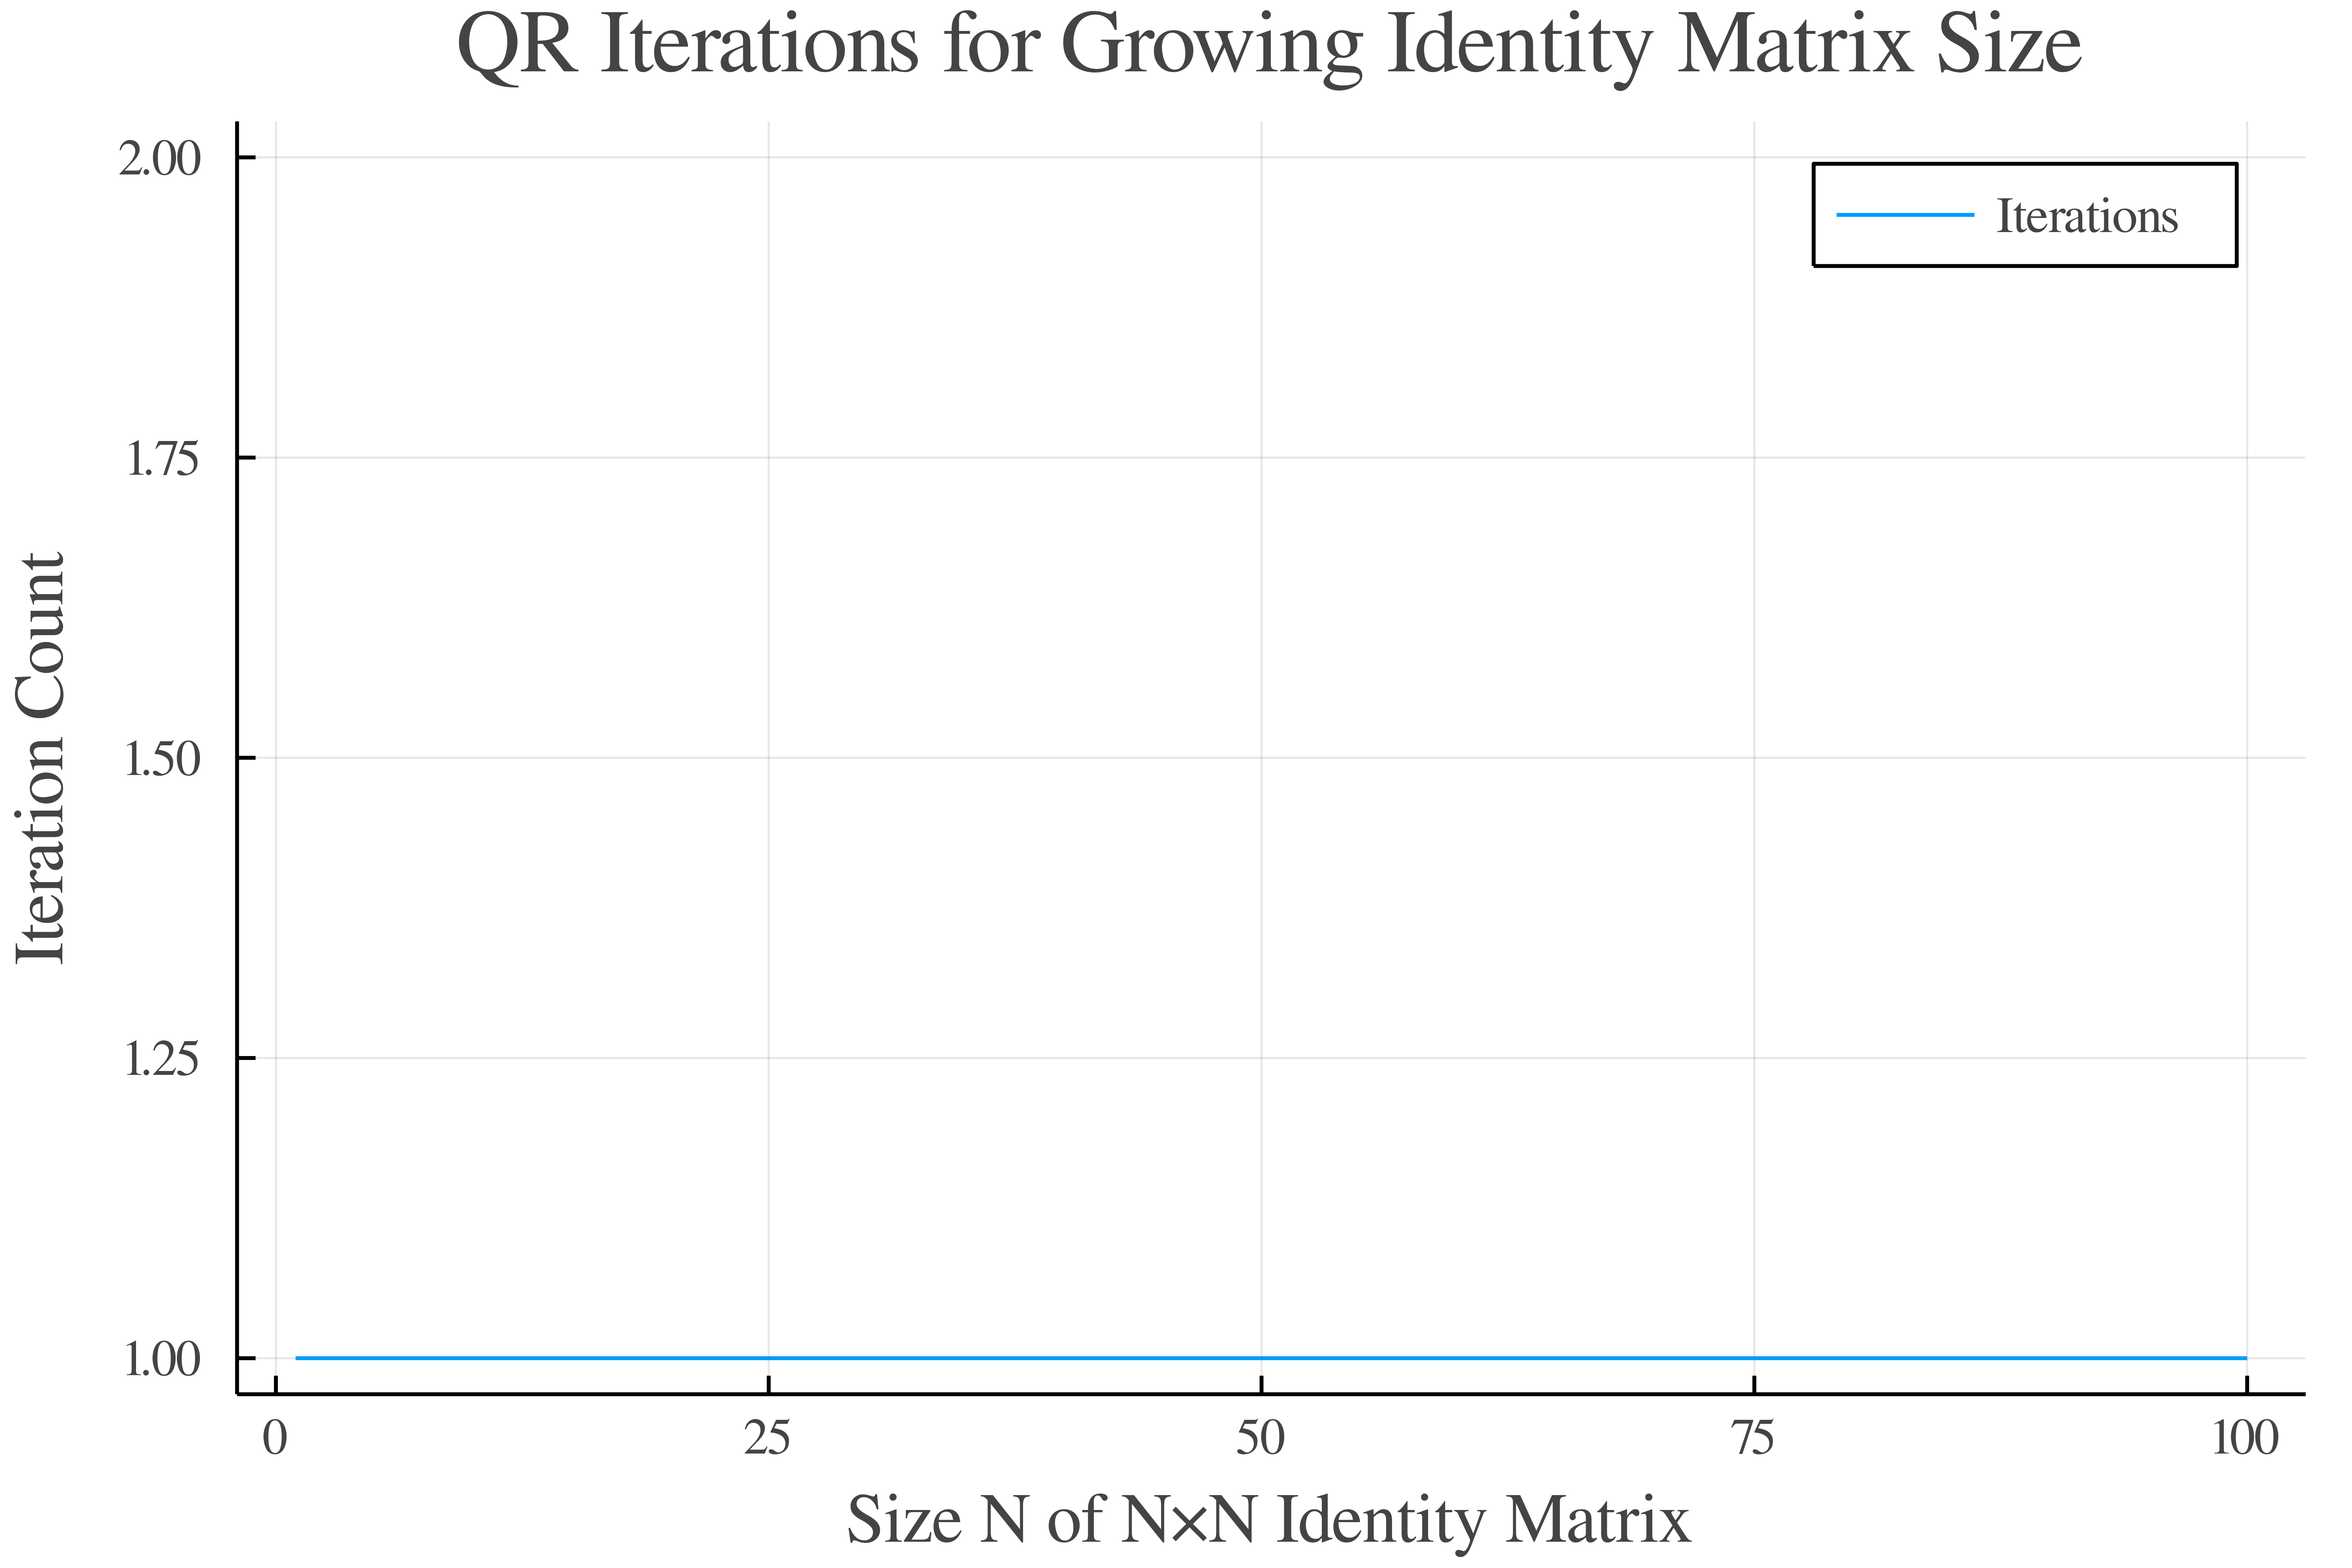
\includegraphics[scale=.055]{graphics/iterations.png}
\caption{A plot of the number of iterations QR took to determine the eigenvalues of the identity matrix of size $N$.}
\end{center}
\end{figure}	

\textbf{Nice Diagonal Matrices and Noise}

In this experiment, I wanted to see how the QR algorithm performs on a diagonal matrix that progressively has more noise added to it. By noise, I mean going from a nice diagonal matrix where all entries are 0 except the diagonal to a diagonal matrix that has noise added to the entire matrix. I have not completed this experiment, since I don't feel I've found interesting results quite yet.
\\

\textit{Source Code}
\begin{lstlisting}
#import necessary libraries
include("../../algorithms/QR_GS.jl")
using LinearAlgebra
using StableRNGs
using Plots
using .QR_GS

#seed for random numbers
rng = StableRNGs.StableRNG(1)

#iterations to perform
iters_todo = 2
nice_size = 15

#to hold iteration count
iterations = zeros(iters_todo)

#create the nice diagonal matrix of size 100,
# simply k = 1, 2, ... 100 along diagonal of 0 matrix
nice = diagm(0 => 1:1:nice_size)

#run this nice matrix through QR algorithm
q1, r1, true_lambdas1, qr_lambdas1, iters1, _ = qr_eigenvals(nice)
iterations[1] = iters1

#progressively add more noise, 10 times
for i = 2:iters_todo
    println("On iteration ", i)
    #generate noise
    noise = i .* rand(rng, nice_size, nice_size)
    #add noise to nice
    noisy = nice + noise
    #run matrix through QR algorithm
    q, r, true_lambdas, qr_lambdas, iters, errors = qr_eigenvals(noisy, 1e-5, 500)
    display(log.(errors))
    #plot for noise level i
    plot(log.(errors),
        xlabel = "Iterations",
        ylabel = "Error between QR and Julia Eigenvalues",
        label = "L2 Norm Difference",
        title = string("QR Error for Noise Level ", i, "x 1e-4"),
        fontfamily = "Times",
        dpi=1000)
    savefig(string("plots/noise_lvl_", i))

    iterations[i] = iters
end
\end{lstlisting}

As of now, I need to find a matrix more interesting than the diagonal one to try the QR algorithm on, since the diagonal one that slowly shifts away from being diagonal seems trivial for the QR algorithm to find the eigenvalues for.

\textbf{Matrices with complex eigenvalues}

Here, I wanted to see how the QR algorithm would react to working on matrices with strictly imaginary eigenvalues. This was before I encounted Francis' discussion on how the algorithm will not succeed on such matrices, so it was interesting to see that for myself first.
\\

\textit{Source Code}
\begin{lstlisting}
#import necessary libraries
include("../../algorithms/QR_GS.jl")
using LinearAlgebra
using Plots
using .QR_GS

##Some matrices to try
#2x2 strictly imaginary eigenvalued matrix, the rotation matrix
rot = [cos(90) -sin(90); sin(90) cos(90)]
m1 = [1 -1; 1 1]
m2 = [4/5 -3/5 0; 3/5 4/5 0; 1 2 2]
m3 = [-1 -4; 1 -1]
m4 = [-3 5; -2 3]

q1, r1, true_lambdas1, qr_lambdas1, iters1, errors1 = qr_eigenvals(rot, 1e-10, 10)
my_display(q1, r1, true_lambdas1, qr_lambdas1, iters1, errors1, "rot")

q2, r2, true_lambdas2, qr_lambdas2, iters2, errors2 = qr_eigenvals(m1, 1e-10, 10)
my_display(q2, r2, true_lambdas2, qr_lambdas2, iters2, errors2, "m1")

q3, r3, true_lambdas3, qr_lambdas3, iters3, errors3 = qr_eigenvals(m2, 1e-10, 10)
my_display(q3, r3, true_lambdas3, qr_lambdas3, iters3, errors3, "m2")

q4, r4, true_lambdas4, qr_lambdas4, iters4, errors4 = qr_eigenvals(m3, 1e-10, 10)
my_display(q4, r4, true_lambdas4, qr_lambdas4, iters4, errors4, "m3")

q5, r5, true_lambdas5, qr_lambdas5, iters5, errors5 = qr_eigenvals(m4, 1e-10, 10)
my_display(q5, r5, true_lambdas5, qr_lambdas5, iters5, errors5, "m4")
\end{lstlisting}

I found that the QR algorithm pretty consistently found the real part of the eigenvalues, but not the complex part.

The following are the outputs I got:
\begin{lstlisting}
true eigenvalues are: 
2-element Vector{ComplexF64}:
 -0.4480736161291702 - 0.8939966636005579im
 -0.4480736161291702 + 0.8939966636005579im
Eigenvalues determined by QR algorithm are: 
2-element Vector{Float64}:
 -0.4480736161291702
 -0.4480736161291702
 
 true eigenvalues are: 
2-element Vector{ComplexF64}:
 1.0 - 1.0im
 1.0 + 1.0im
Eigenvalues determined by QR algorithm are: 
2-element Vector{Int64}:
 1
 1
 
 true eigenvalues are: 
3-element Vector{ComplexF64}:
 0.8 - 0.6000000000000001im
 0.8 + 0.6000000000000001im
 2.0 + 0.0im
Eigenvalues determined by QR algorithm are: 
3-element Vector{Float64}:
 0.8
 0.8
 2.0
 
 true eigenvalues are: 
2-element Vector{ComplexF64}:
 -1.0 - 2.0000000000000004im
 -1.0 + 2.0000000000000004im
Eigenvalues determined by QR algorithm are: 
2-element Vector{Int64}:
 -1
 -1
 
 true eigenvalues are: 
2-element Vector{ComplexF64}:
 2.42861286636753e-16 - 1.0000000000000004im
 2.42861286636753e-16 + 1.0000000000000004im
Eigenvalues determined by QR algorithm are: 
2-element Vector{Int64}:
 -3
  3
\end{lstlisting}

It was interesting seeing that the QR algorithm was pretty inaccurate on the final matrix. This is something I plan on looking further into.

\bibliography{references} % Delete if no references
% See woc_2col.text for how to cite sources

 \begin{thebibliography}{9}
 %
 % and use \bibitem to create references.
 %

\bibitem{RefA}
J.G.F. Francis, "The QR Transformation, I", The Computer Journal, 4(3), pages 265–271 (1961, received October 1959) online at oxfordjournals.org

\bibitem{RefB}
Leon, S.J., Björck, Å. and Gander, W. (2013), Gram-Schmidt orthogonalization: 100 years and more. Numer. Linear Algebra Appl., 20: 492-532. https://doi.org/10.1002/nla.1839

\bibitem{RefC}
A. S. HOUSEHOLDER (1958), A class of methods for inverting matrices. J. Soc. Ind. Appl. Math. 6, 189-195.

\bibitem{RefD}
Bindel, D.; Demmel, J.; Kahan, W.; Marques, O. (2000), On Computing Givens rotations reliably and efficiently. LAPACK Working Note 148, University of Tennessee, UT-CS-00-449, January 31, 2001.

\bibitem{RefE}
J. G. F. Francis, The QR Transformation—Part 2, The Computer Journal, Volume 4, Issue 4, 1962, Pages 332–345, https://doi.org/10.1093/comjnl/4.4.332

 \end{thebibliography}

\end{document}